\everymath{\displaystyle}
\documentclass{beamer}
% \documentclass[handout]{beamer}

%\usepackage[pdftex]{color,graphicx}
\usepackage{amsmath,amssymb,amsfonts}

\mode<presentation>
{
  % \usetheme{Darmstadt}
  % \usetheme[hideothersubsections]{Hannover}
  % \usetheme[hideothersubsections]{Goettingen}
  \usetheme[hideothersubsections, right]{Berkeley}

  \usecolortheme{seahorse}
  % \usecolortheme{dolphin}
  \usecolortheme{rose}
  % \usecolortheme{orchid}

  \useinnertheme[shadow]{rounded}

  % \setbeamercovered{transparent}
  \setbeamercovered{invisible}
  % or whatever (possibly just delete it)
}

\mode<handout>{
  \setbeamercolor{background canvas}{bg=black!5}
  \usepackage{pgfpages}
  \pgfpagesuselayout{4 on 1}[a4paper,border shrink=5mm, landscape]
}

\usepackage[brazilian]{babel}
% or whatever

% \usepackage[latin1]{inputenc}
\usepackage[utf8]{inputenc}
% or whatever

\usepackage{times}
%\usepackage[T1]{fontenc}
% Or whatever. Note that the encoding and the font should match. If T1
% does not look nice, try deleting the line with the fontenc.


\title[Significância] % (optional, use only with long paper titles)
{Significância Estatística}

\subtitle
{O p-valor e Testes de Hipóteses} % (optional)

\author%[] % (optional, use only with lots of authors)
{Felipe Figueiredo}% \and S.~Another\inst{2}}
% - Use the \inst{?} command only if the authors have different
%   affiliation.

\institute[] % (optional, but mostly needed)
{
}
  % \inst{1}%
  % Department of Computer Science\\
  % University of Somewhere
  % \and
  % \inst{2}%
  % Department of Theoretical Philosophy\\
  % University of Elsewhere}
% - Use the \inst command only if there are several affiliations.
% - Keep it simple, no one is interested in your street address.

\date%[] % (optional)
{}

% \subject{Talks}
% This is only inserted into the PDF information catalog. Can be left
% out. 



% If you have a file called "university-logo-filename.xxx", where xxx
% is a graphic format that can be processed by latex or pdflatex,
% resp., then you can add a logo as follows:

\pgfdeclareimage[height=1.6cm]{university-logo}{../logo}
\logo{\pgfuseimage{university-logo}}



% Delete this, if you do not want the table of contents to pop up at
% the beginning of each subsection:
\AtBeginSubsection[]
%\AtBeginSection[]
{
  \begin{frame}<beamer>{Sumário}
    \tableofcontents[currentsection,currentsubsection]
  \end{frame}
}


% If you wish to uncover everything in a step-wise fashion, uncomment
% the following command: 

% \beamerdefaultoverlayspecification{<+->}


\begin{document}

\begin{frame}
  \titlepage
\end{frame}

\begin{frame}{Sumário}
  \tableofcontents
  % You might wish to add the option [pausesections]
\end{frame}


%% Template
% \section{}

% \subsection{}

% \begin{frame}{}
%   \begin{itemize}
%   \item 
%   \end{itemize}
% \end{frame}

% \begin{frame}
%   \begin{columns}
%     \begin{column}{5cm}
%     \end{column}
%     \begin{column}{5cm}
%     \end{column}
%   \end{columns}
% \end{frame}

% \begin{frame}{}
%   \includegraphics[height=0.4\textheight]{file1}
%   \includegraphics[height=0.4\textheight]{file2}
%   \includegraphics[height=0.4\textheight]{file3}
%   \begin{figure}
%     \caption{}
%   \end{figure}
% \end{frame}

% \begin{frame}{}
%   \begin{definition}
%   \end{definition}
%   \begin{example}
%   \end{example}
%   \begin{block}{Exercício}
%   \end{block}
% \end{frame}

% \section{O p-valor}

\section{Discussão da aula passada}

\subsection{Discussão da aula passada}

\begin{frame}{Discussão da aula passada}
  \begin{block}{}
    Discussão da leitura obrigatória da aula passada
  \end{block}
\end{frame}

\section{Testes de Hipóteses}

\subsection{Hipóteses}

\begin{frame}{Introdução}
  \begin{block}{Abertura de ``A Divina Comédia''}
    \small
    {\em ``A meio do caminho, ou seja, da duração expectável de sua vida, Dante, consciente de se haver desviado do reto procedimento, encontra-se perdido numa alegórica 'Selva Perdida'.

      \bigskip
      Encontra aí a figura de Virgílio, o poeta latino que (...) vem se lhe oferecer como guia para o Inferno e o Purgatório onde, pelo exemplo dos pecadores e de suas penas, Dante poderá encontrar o caminho da sua salvação.''}
  \end{block}
\hfill Dante Alighieri
\end{frame}

\begin{frame}{Hipóteses científicas}
  \begin{itemize}
  \item Podemos tomar decisões baseado nos dados de um experimento
    (amostra).
  \item Para isto, precisamos de um critério sistemático e rigoroso
    que possa aferir o quanto os dados suportam esta decisão.
  \item Usando os conceitos de probabilidades, poderemos ainda
    calcular a probabilidade de que esta decisão esteja errada.
  \end{itemize}
  \begin{block}{}
    {\bf Hipóteses devem ser falseáveis, portanto formuladas como afirmações}.
  \end{block}
\end{frame}

\begin{frame}{Exemplo 1}
  \begin{exampleblock}{Exemplo 1}
    \footnotesize
    Um neurologista está testando o efeito de uma droga no tempo de
    resposta de um certo estímulo neurológico.
    Para isto, ele injeta uma dose da droga em 100 ratos, cria
    os estímulos neurológicos e observa o tempo de resposta em cada
    animal.

    \smallskip
    O neurologista sabe que o tempo de resposta médio de ratos que não
    receberam a droga é de 1.2 segundos.

    \smallskip
    O tempo de resposta médio dos ratos injetados foi de
    1.05 segundos, com desvio padrão amostral de
    0.5 segundos.
  \end{exampleblock}
  \begin{block}{}
    Você acha que a droga tem efeito no tempo de resposta do estímulo?
  \end{block}
  \hfill {\scriptsize Fonte: Khan Academy}
\end{frame}

\begin{frame}[label=exemplo1]{Exemplo 1}
  \begin{exampleblock}{Exemplo 1}
    \footnotesize
    Um neurologista está testando o efeito de uma droga no tempo de
    resposta de um certo estímulo neurológico.
    Para isto, ele injeta uma dose da droga em \alert{100} ratos, cria
    os estímulos neurológicos e observa o tempo de resposta em cada
    animal.

    \smallskip
    O neurologista sabe que o tempo de resposta médio de ratos que não
    receberam a droga é de \alert{1.2 segundos}.

    \smallskip
    O tempo de resposta médio dos ratos injetados foi de
    \alert{1.05 segundos}, com desvio padrão amostral de
    \alert{0.5 segundos}.
  \end{exampleblock}
  \begin{block}{}
    {\bf Você acha que a droga tem efeito no tempo de resposta do estímulo?}
  \end{block}
  \hfill {\scriptsize Fonte: Khan Academy}
\end{frame}

\begin{frame}{Exemplo 1}
  \begin{exampleblock}{Exemplo 1}
    \footnotesize
    Um neurologista está testando o efeito de uma droga no tempo de
    resposta de um certo estímulo neurológico.
    Para isto, ele injeta uma dose da droga em \alert{100} ratos, cria
    os estímulos neurológicos e observa o tempo de resposta em cada
    animal.

    \smallskip
    O neurologista sabe que o tempo de resposta médio de ratos que não
    receberam a droga é de \alert{1.2 segundos}.

    \smallskip
    O tempo de resposta médio dos ratos injetados foi de
    \alert{1.05 segundos}, com desvio padrão amostral de
    \alert{0.5 segundos}.
  \end{exampleblock}
  \begin{block}{}
    Você tem informações suficientes para construir um IC em torno de $\bar{x}$?
  \end{block}
  \hfill {\scriptsize Fonte: Khan Academy}
\end{frame}

\begin{frame}{Análise Inferencial}
  \begin{exampleblock}{Exemplo 1}
    \scriptsize
    Um neurologista está testando o efeito de uma droga no tempo de
    resposta de um certo estímulo neurológico.

    \smallskip
    Tempo de resposta típico = \alert<2->{1.2 s}.

    \smallskip
    $n$ = \alert{100}

    $\bar{x}$ = \alert{1.05 s}

    $s$ = \alert{0.5 s}

  \end{exampleblock}
  \uncover<1->{\begin{exampleblock}{IC da média}
      \small
      IC = 0.9508 até 1.1492
   \end{exampleblock}}
 \uncover<2>{\begin{exampleblock}{IC da diferença entre $\bar{x}$ e 1.2}
      \small
     $\bar{d}$ = -0.1500, IC = -0.2492 até -0.0508
   \end{exampleblock}}
 % \hfill{\scriptsize calculado em \url{https://www.graphpad.com/quickcalcs/oneSampleT2/}}
\end{frame}

\begin{frame}{Teste de Significância}
  \begin{exampleblock}{Exemplo 1}
    \scriptsize
    Um neurologista está testando o efeito de uma droga no tempo de
    resposta de um certo estímulo neurológico.

    \smallskip
    Tempo de resposta típico = \alert{1.2 s}.

    \smallskip
    $n$ = \alert{100}

    $\bar{x}$ = \alert{1.05 s}

    $s$ = \alert{0.5 s}

  \end{exampleblock}
  \begin{exampleblock}{Teste de significância entre $\bar{x}$ e 1.2}
      \small
     p = 0.0034
   \end{exampleblock}

   \begin{center}
     \small
     É hoje!
   \end{center}
 % \hfill{\scriptsize calculado em \url{https://www.graphpad.com/quickcalcs/oneSampleT2/}}
\end{frame}

\begin{frame}{Hipóteses estatísticas}
  \begin{block}{Definição}
    \small
    Em Estatística, uma \alert{hipótese} é uma afirmação sobre uma
    característica de uma população, tipicamente o valor de um
    parâmetro.
  \end{block}
  \begin{block}{Definição}
    \small
    Um \alert{teste de hipóteses} (ou teste de significância) é um
    procedimento sistemático para testar uma afirmação sobre uma
    característica de uma população.
  \end{block}
\end{frame}

\begin{frame}{Pergunta}
  \begin{exampleblock}{Exemplo 1}
    \scriptsize
    Um neurologista está testando o efeito de uma droga no tempo de
    resposta de um certo estímulo neurológico.

    \smallskip
    Tempo de resposta típico = \alert{1.2 s}.

    \smallskip
    $n$ = \alert{100}

    $\bar{x}$ = \alert{1.05 s}

    $s$ = \alert{0.5 s}
  \end{exampleblock}
  \begin{block}{Pense...}
    \uncover<1>{Que possíveis conclusões você pode chegar com esse experimento?}

    \bigskip
    \uncover<2>{Como você formularia a hipótese do exemplo anterior?}
  \end{block}
\end{frame}

\begin{frame}{Identificando hipóteses}
  \begin{block}{}
    \small
    Uma hipótese estatística deve ser testável frente a dados obtidos de um experimento.
  \end{block}
  \begin{exampleblock}{Exemplo 1}
    \footnotesize
    O tempo de resposta dos ratos que receberam a droga é menor que 1.2s.
  \end{exampleblock}
  \begin{exampleblock}{{\footnotesize Exemplo}}
    \scriptsize
    Um jornalista alega que a maior parte dos motoristas atravessa o
    sinal vermelho.
  \end{exampleblock}
  \begin{exampleblock}{{\footnotesize Exemplo}}
    \scriptsize
    Pesquisadores afirmam que a temperatura corporal média de adultos
    sadios não ultrapassa 37$^o$C.
  \end{exampleblock}
\end{frame}

\begin{frame}{Identificando hipóteses}
  \begin{block}{1 teste = 2 hipóteses}
    Um teste de hipóteses envolve a formulação de uma {\em hipótese nula} e uma {\em hipótese alternativa}.
  \end{block}
  \begin{itemize}
    \small
    \bigskip
  \item A hipótese nula ($H_0$) é a hipótese que não há efeito real.
    \bigskip
  \item A hipótese alternativa ($H_1$ ou $H_a$) é a de que há efeito real \alert{que pode ser detectado} com o experimento.
    \begin{itemize}
    \item Obs: (em geral) hipótese de interesse científico
    \end{itemize}
.
  \end{itemize}
\end{frame}

\begin{frame}{Atenção}
  \begin{block}{{\em Danger Will Robinson...}}
    A lógica do teste de hipóteses é o \alert{inverso} do que se esperaria inuitivamente.

    \bigskip
    Isto é, ao invés de testar a hipótese de interesse, vamos {\em testar a hipótese nula} -- e tentar rejeitá-la.
  \end{block}

  \hfill
  \begin{center}
    {\bf Mantenha isso em mente daqui a para a frente.}
  \end{center}
\end{frame}

\begin{frame}{Identificando hipóteses}
  \begin{block}{Roteiro}
    \begin{enumerate}
    \item Identificar a afirmação a ser testada e expressá-la em forma simbólica
    \item Expressar em forma simbólica a afirmação que deve ser
      verdadeira, caso a afirmação de interesse seja falsa
    % \item Das duas expressões obtidas, a hipótese $H_0$ será a que
    %   contém igualdade $=$, enquanto a $H_1$ será a que contém um
    %   sinal de $<$, $>$ ou $\ne$.
    \end{enumerate}
  \end{block}
\end{frame}

\begin{frame}{{\footnotesize Quais são as variáveis?}}
  \begin{exampleblock}{Exemplo 1}
    \scriptsize
    Um neurologista está testando o efeito de uma droga no tempo de
    resposta de um certo estímulo neurológico.

    \smallskip
    Tempo de resposta típico = \alert{1.2 s}.

    \smallskip
    $n$ = \alert{100}

    $\bar{x}$ = \alert{1.05 s}

    $s$ = \alert{0.5 s}
  \end{exampleblock}
  \begin{block}{Modelo}<2->
    \begin{displaymath}
      \text{variável dependente} \sim \text{variável independente}
    \end{displaymath}
    \begin{displaymath}
      \text{tempo de resposta} \sim \text{ratos injetados com a droga}
    \end{displaymath}
  \end{block}
\end{frame}

\begin{frame}{{\footnotesize Quais são as hipóteses estatísticas?}}
  \begin{exampleblock}{Exemplo 1}
    \scriptsize
    Um neurologista está testando o efeito de uma droga no tempo de
    resposta de um certo estímulo neurológico.

    \smallskip
    Tempo de resposta típico = \alert{1.2 s}.

    \smallskip
    $n$ = \alert{100}

    $\bar{x}$ = \alert{1.05 s}

    $s$ = \alert{0.5 s}
  \end{exampleblock}
  \begin{exampleblock}{Hipóteses}<2->
    \begin{displaymath}
      H_0: \mu=1.2
    \end{displaymath}
    \begin{displaymath}
      H_1: \mu \ne 1.2
    \end{displaymath}
  \end{exampleblock}
\end{frame}

\begin{frame}{Identificando hipóteses}
  \begin{exampleblock}{Exemplo}
    Formulação verbal:\\
    A proporção de motoristas que admitem atravessar o sinal vermelho
    é maior que 50\%.\\
    \bigskip
    Formulação matemática:\\
    \begin{displaymath}
      H_0: p=0.5
    \end{displaymath}
    \begin{displaymath}
      H_1: p>0.5
    \end{displaymath}
  \end{exampleblock}
\end{frame}

\begin{frame}{Identificando hipóteses}
  \begin{exampleblock}{Exemplo}
    Formulação verbal:\\
    A altura média de jogadores profissionais de basquete é de no
    máximo 2.20m.\\
    \bigskip
    Formulação matemática:\\
    \begin{displaymath}
      H_0: \mu = 2.20
    \end{displaymath}
    \begin{displaymath}
      H_1: \mu < 2.20
    \end{displaymath}
  \end{exampleblock}
\end{frame}

\begin{frame}{Identificando hipóteses}
  \begin{exampleblock}{Exemplo}
    Formulação verbal:\\
    A dose média contida em um comprimido de paracetamol é de 750mg.\\
    \bigskip
    Formulação matemática:\\
    \only<1>{\begin{displaymath}
      H_0: \mu = 750
    \end{displaymath}}
    \only<2>{\alert{\begin{displaymath}
      H_0: \mu = 750
    \end{displaymath}}}
    \begin{displaymath}
      H_1: \mu \ne 750
    \end{displaymath}
  \end{exampleblock}
  \begin{center}
      \uncover<2->{
\includegraphics[height=2cm]{Cap10-11/Jackie-Chan-WTF}}
  \end{center}
\end{frame}

\begin{frame}{Identificando a região crítica}
  Em geral...
  \begin{itemize}
  % \item Para identificar a região crítica (ou região de rejeição) do
  %   teste, devemos observar se o teste é unicaudal (à esquerda ou à
  %   direita) ou bicaudal.
  \item Se $H_1$ é do tipo $\ne$, o teste é bicaudal (ou bilateral).
  \item Se $H_1$ é do tipo $<$, o teste é unicaudal (ou unilateral) à esquerda.
  \item Se $H_1$ é do tipo $>$, o teste é unicaudal à direita.
  \end{itemize}
\end{frame}

\subsection{Significância}
\begin{frame}{Significância}
  \begin{itemize}
  \item A {\bf significância} do estudo deve ser arbitrada antes do experimento (planejamento)
  \item Está associada aos erros induzidos pela variabilidade experimental
  \item Ou seja, mesmo fazendo tudo certo, você pode ser induzido a chegar numa conclusão errada ao acaso!
  \item Isso pode ocorrer de duas maneiras diferentes...
  \end{itemize}
\end{frame}

\begin{frame}{Tipos de erros em testes de hipóteses}
  \begin{block}{Definição}
    Um \alert{erro do tipo I} ocorre se a hipótese nula for rejeitada
    quando é verdadeira.
  \end{block}
  \begin{block}{Definição}
    Um \alert{erro do tipo II} ocorre se a hipótese não for rejeitada
    quando for falsa.
  \end{block}
\end{frame}

\begin{frame}{Observe}
  \begin{block}{A questão importante aqui é:}
    MESMO SE a hipótese nula {\bf for verdadeira}, ainda assim você pode observar (ao acaso) uma diferença como resultado do experimento.

    \bigskip
    (ex., muita variabilidade, amostras pequenas, etc.).

    \bigskip
    {\bf Isso} é o erro tipo I. Trabalhamos para que isso seja raro (não mais que 5\% das vezes).
  \end{block}
\end{frame}

\begin{frame}{Tipos de erros em testes de hipóteses}
  \begin{block}{}
    \begin{tabular}{c||c|c}
      Decisão / Verdade & $H_0$ é verdadeira & $H_0$ é falsa \\
      \hline
      \hline
      Não rejeitar $H_0$ & Decisão correta & Erro do tipo II\\
      \hline
      Rejeitar $H_0$ & Erro do tipo I & Decisão correta\\
    \end{tabular}
  \end{block}
  \begin{itemize}
  \item Erro do tipo I = falso positivo
  \item Erro do tipo II = falso negativo
  \end{itemize}
\end{frame}

\begin{frame}{Nível de significância}
  \begin{block}{Definição}
    O \alert{nível de significância} de um teste de hipótese é sua
    probabilidade máxima admissível para cometer um erro do tipo
    I. Ele é denotado por $\alpha$.

    \bigskip
    Está associado com o nível de confiança.
  \end{block}
  \begin{block}{Definição}
    A probabilidade de se cometer um erro do tipo II é denotada por
    $\beta$.

    \bigskip Está associado com o poder estatístico do teste (futuro).
  \end{block}
  % \begin{itemize}
  % % \item O valor $1-\beta$ é chamado o \alert{poder do teste}.
  % % \item Devemos controlar o erro do tipo I, isto é, 
  % % \item Quando você decresce $\alpha$, você provavelmente aumentará $\beta$.
  % \end{itemize}
\end{frame}

\begin{frame}{Componentes de um teste de hipóteses}
  São necessários para um teste de hipóteses:
  \begin{itemize}
  \item As hipóteses nula e alternativa
  \item O nível de significância
  \item A região crítica (tipo de teste)
  \item A estatística de teste (softwares especializados)
%  \item 
  \end{itemize}
  \begin{block}{Observação}
    O teste unicaudal {\bf divide} a probabilidade de erro à esquerda (valores menores) e à direita (valores maiores).

    \bigskip
    Assim, 5\% de significância num teste unicaudal corresponde à 2.5\% (metade) da significância bicaudal.

    \bigskip
    Mais detalhes no cap 10.
  \end{block}
\end{frame}

\begin{frame}{Rejeitar hipóteses}
  \begin{block}{Importante}
    Observe que o teste de hipótese nunca deve \alert{aceitar} uma
    hipótese nula, apenas rejeitá-la ou deixar de rejeitá-la.
  \end{block}
\end{frame}

\subsection{O p-valor}

\begin{frame}{O p-valor}
  \begin{block}{Definição}
    Assumindo que a hipótese nula seja verdadeira, o {\bf p-valor} de
    um teste de hipóteses é a probabilidade de se obter uma
    estatística amostral com valores \alert{tão extremos, ou mais
      extremos} que aquele observado.
  \end{block}

  O p-valor \alert{é}:
  \begin{itemize}
    \footnotesize
  % \item Uma estatística (i.e., depende da amostra - dados e tamanho)
  \item A probabilidade (condicional) de se observar o resultado ao
    acaso \alert{dado que} a $H_0$ é verdadeira.
  \item Uma medida da força da evidência \alert{contra} a $H_0$.
  \end{itemize}
\end{frame}

\begin{frame}{O p-valor}
  \begin{block}{Como utilizar}
    \begin{itemize}
    \item Quanto menor o p-valor, mais evidências para rejeitar a
      hipótese nula.
    \item O ponto de corte mais utilizado é a significância de 5\%
    \item Assim, qualquer $p \le 0.05$ é estatisticamente significante.
    \end{itemize}
  \end{block}
\end{frame}

% \begin{frame}{O p-valor}
%   \begin{figure}
%     \centering
%       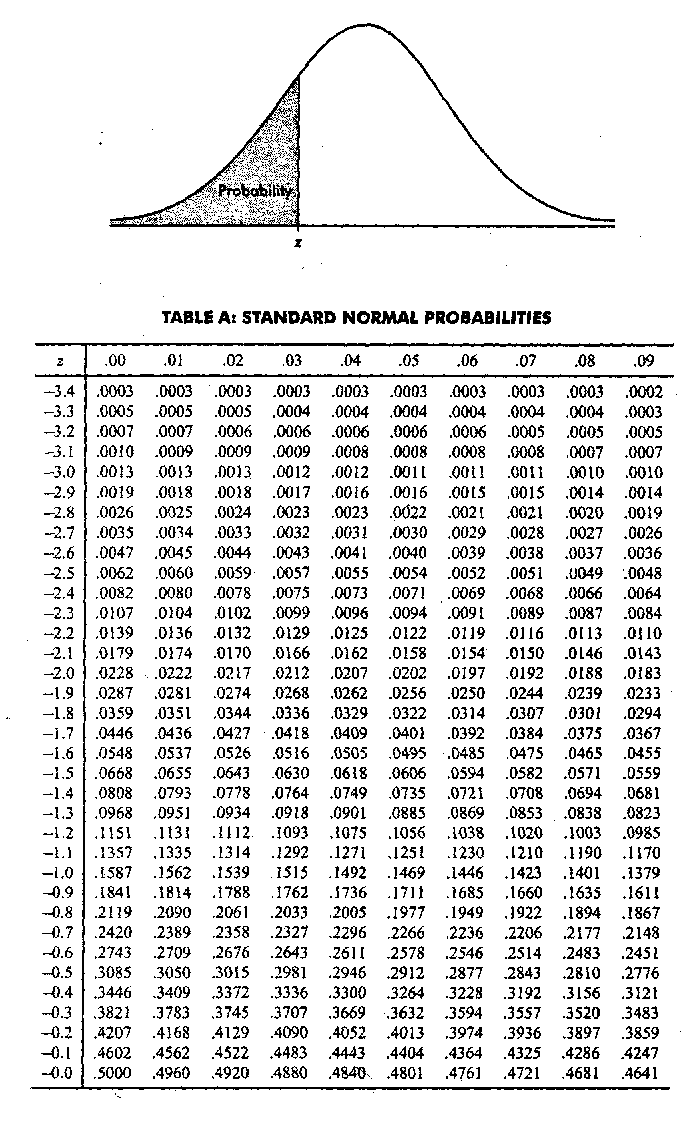
\includegraphics[height=0.9\textheight]{TH_II/z_table}
%   \end{figure}
% \end{frame}

\againframe{exemplo1}

\begin{frame}{Exemplo 1}
  \begin{block}{Pense...}
    \begin{itemize}
    \item A hipótese científica é que a droga afeta o tempo de resposta.
    \item Como você formularia a hipótese estatística ($H_1$)?
      \begin{enumerate}
      \item $H_0: \mu = 1.2, H_1: \mu \ge 1.2$ (teste unicaudal à direita)
      \item $H_0: \mu = 1.2, H_1: \mu < 1.2$ (teste unicaudal à esquerda)
      \item \alert<2>{$H_0: \mu = 1.2, H_1: \mu \ne 1.2$ (teste bicaudal)}
      \item $H_0: \mu \ge 1.2, H_1: \mu = 1.2$ (teste unicaudal à esquerda)
      \end{enumerate}

      Resposta: \only<2->{\bf Opção 3}
%    \item Qual seria a hipótese nula ($H_0$) a ser rejeitada, caso a droga seja eficaz?
    \end{itemize}
  \end{block}
\end{frame}

\begin{frame}{Exemplo 1}
  % \begin{exampleblock}{Exemplo 1}
    \begin{itemize}
      \scriptsize
    \item Dados: $\mu = 1.2, \bar{x} = 1.05, s = 0.5, n=100$
    \item $\alert<2->{H_0: \mu = 1.2}, H_1: \mu \ne 1.2$ (teste bicaudal)
    % \item $n$ é grande ($n > 30$), então usamos $\sigma \approx s$ , e
    %   fazemos o teste Z:
    % \item $Z = \frac{1.05 - 1.2}{\frac{0.5}{\sqrt{100}}} = -3$
      \begin{itemize}
        \scriptsize
      \item O teste Z retorna $p = 0.0027$\footnote{Premissas fortes: Normal, N grande, $\sigma$ conhecido, etc.}
      \item O teste t retorna $p = 0.0034$\footnote{Usado em geral, menos premissas}
      \end{itemize}
    \item<2-> Como $p < 0.05$, há evidências para rejeitar \alert<2->{$H_0$}.
    \end{itemize}
  % \end{exampleblock}
  \begin{exampleblock}{Resultado}<3->
    \small
    O tempo de resposta médio é \alert{significativamente} diferente de 1.2 s ({\footnotesize p = 0.0034}).
  \end{exampleblock}
  \begin{exampleblock}{Conclusão}<4->
    \small
    (...) há evidências que a droga altera o tempo (...)  de resposta (...).
  \end{exampleblock}

   % \hfill{\scriptsize teste Z calculado em \url{https://mathcracker.com/z-test-for-one-mean.php}
\end{frame}

\begin{frame}{Cuidados com o p-valor}
    \begin{block}{{\small DOREY, F. 2010 Clin Orthop Relat Res.}}
    \small
    {\em ``The concept of a p value is not simple and any statements
    associated with it must be considered cautiously.''}
  \end{block}
\end{frame}

\begin{frame}{Cuidado!}
  \small
  \begin{block}{O p-valor \alert{não é}}
    \begin{itemize}
      \footnotesize
    \item a probabilidade de que a hipótese nula seja verdadeira
    \item a probabilidade de que a diferença observada seja devido ao
      acaso
    \end{itemize}
  \end{block}
  \begin{center}
    Estes são erros comuns de interpretação
  \end{center}
  \begin{block}{O p-valor assume que...}
    \small
    \begin{enumerate}
      \footnotesize
    \item a hipótese é verdadeira
    \item que a \alert{única} causa da diferença é devida ao acaso,
    \end{enumerate}
    \begin{center}
      Portanto não pode ser usado para concluir suas próprias
      premissas.
    \end{center}
  \end{block}
\end{frame}

\subsection{Exercício}

\begin{frame}{Exercício}
  \begin{exampleblock}{Exemplo 2}
    \footnotesize
    Uma indústria farmacêutica especifica que em certo analgésico a
    quantidade média de ácido acetil salicílico deve ser 5.5 gramas
    por comprimido. A indústria suspeita que houve problemas na
    produção de um determinado lote e que, nesse lote, a quantidade
    média dessa substância está diferente da especificada. Para
    verificar essa suspeita, a indústria selecionou uma amostra
    aleatória de 40 comprimidos desse lote, observando uma quantidade
    média de ácido acetil salicílico igual a 5.2 gramas e um desvio
    padrão de 0.7 gramas.
  \end{exampleblock}
  \begin{block}{Pergunta}<2>
    Você tem informações suficientes para executar um teste formal de hipóteses?

    Em caso afirmativo, formule a $H_0$ e a $H_1$.
  \end{block}
\end{frame}

% \begin{frame}{Exemplo 2}
%   \begin{itemize}
%   % \item Para testar essa hipótese usaremos o teste Z pois a amostra é
%   %   grande ($n=40$).
%   \item O teste é bicaudal, portanto consultamos a significância
%     \alert{$\frac{\alpha}{2} = 0.025$}.
%   \item Consultando a tabela Z, encontramos o valor crítico
%     \alert{$z_{0.025} = 1.96$}.
%   \item Após calcular a estatística de teste, devemos comparar com o
%     valor crítico $z_c$ para verificar se ela está contida na região
%     de rejeição.
%   \end{itemize}
% \end{frame}

\begin{frame}{Exemplo 2}
  \begin{exampleblock}{Resposta}
    \begin{itemize}
    \footnotesize
  \item Temos as informações necessárias para o teste
  \item Hipóteses
      \begin{displaymath}
        H_0: \mu = 5.5
      \end{displaymath}
      \begin{displaymath}
        H_1: \mu \ne 5.5
      \end{displaymath}
    % \item Região crítica: $z<-z_{0.025}$ ou $z>z_{0.025}$ (ou seja,
    %   \alert{$z<-1.96$ ou $z>1.96$}).
    \item Dados
      \begin{displaymath}
        n=40, \bar{x} = 5.2, s = 0.7
      \end{displaymath}
    % \item Estatística de teste
    %   \begin{displaymath}
    %     z = \frac{5.2 - 5.5}{\frac{0.7}{\sqrt{1000}}} = \alert{-2.71}
    %   \end{displaymath}
    \end{itemize}
  \end{exampleblock}
  \begin{exampleblock}{Solução}<2>
    p = 0.0099
  \end{exampleblock}
\end{frame}

\begin{frame}{Exemplo 2}
  \begin{block}{Interpretação}
    \scriptsize

    A probabilidade de observarmos ao acaso um valor tão discrepante
    como 5.2 g ou mais é menor que o nível de significância
    estabelecido $\alpha=0.05$.

    \bigskip
    Rejeitamos a hipótese de que a quantidade média é igual a 5.5 g ao
    nível de significância de 5\%.
  \end{block}
  \begin{exampleblock}{Resultado}<2->
    \footnotesize

    (...) a dose média de ácido acetil salicílico (em gramas por
    comprimido) de certo analgésico é significativamente diferente de
    5.5 g (p = 0.0099).
  \end{exampleblock}
  \begin{exampleblock}{Conclusão}<3->
    O lote (...)
    % deste medicamento
    está fora da especificação de 5.5 g (...) por comprimido,
    portanto o lote está reprovado.
  \end{exampleblock}
\end{frame}

\begin{frame}{Bônus: Intervalo de Confiança}
  \begin{itemize}
  \item Nessa situação, podemos usar o intervalo de confiança para
    realizar o teste de hipóteses, pois a hipótese alternativa é
    bilateral.
  \item Como queremos um teste a 5\% de significância, calcularemos um
    intervalo de 95\% de confiança para a quantidade média de ácido
    acetil salicílico, por comprimido.
  \end{itemize}
\end{frame}

\begin{frame}{Exemplo 2 (a revanche)}
  \begin{exampleblock}{IC da média}
    \begin{itemize}
      \scriptsize
    \item Dados: $n=40, \bar{x} = 5.2, s = 0.7$
    \item IC: [4.976, 5.424] $\approx$ [5.0, 5.4]
    \end{itemize}
    % média p <  0.0001
    % The difference between these two values is 5.200
    % The   95% confidence interval of this difference:
    % From 4.976 to 5.424
  \end{exampleblock}
  \begin{exampleblock}{Resultado}<2->
    \footnotesize
    A quantidade média neste lote (...)
    % de ácido acetil salicílico, por comprimido,
    está entre 5.0 e 5.4 gramas, com 95\% de confiança.
  \end{exampleblock}
  \begin{block}{Interpretação}<2->
    \footnotesize
    A ``meta'' 5.5 g não está contida no IC.
  \end{block}
  \begin{exampleblock}{Conclusão}<3->
    (...), portanto o lote está reprovado.
  \end{exampleblock}
\end{frame}

\begin{frame}{Exemplo 2 (a revanche)}
  \begin{exampleblock}{IC da média}
    \begin{itemize}
      \scriptsize
    \item Dados: $n=40, \bar{d} = 5.2, s = 0.7, \mu = 5.5$
    \item $\bar{d} = -0.300$, IC: [-0.524, -0.076] $\approx$ [-0.5, -0.1]
    \end{itemize}
    % Diferença
    % The difference between these two values is -0.300
    % The   95% confidence interval of this difference:
    % From -0.524 to -0.076
  \end{exampleblock}
  \begin{exampleblock}{Resultado}
    \footnotesize
    A diferença média neste lote (...)
    % de ácido acetil salicílico, por comprimido,
    está entre -0.5 e -0.1 gramas, com 95\% de confiança.
  \end{exampleblock}
  \begin{block}{Interpretação}
    \footnotesize
    A ``meta de igualdade'' $d = 0$ g não está contida no IC.
  \end{block}
  \begin{exampleblock}{Conclusão}
    (...), portanto o lote está reprovado.
  \end{exampleblock}
\end{frame}

% \begin{frame}{Interpretação do IC}
%   \begin{block}{Interpretação}
%     A quantidade média de ácido acetil salicílico, por comprimido,
%     está entre 5,0 e 5,4 gramas, com 95\% de confiança.
%   \end{block}
%   \begin{itemize}
%   \item Teste de hipóteses baseado no intervalo de confiança: o valor
%     5.5 não pertence ao intervalo de 95\% de confiança para a
%     quantidade média de ácido acetil salicílico, por comprimido.
%   \item Conclusão: rejeitamos a hipótese de que a quantidade média de
%     ácido acetil salicílico de certo analgésico é igual a 5.5 gramas
%     ao nível de significância de 5\%.
%   \end{itemize}
% \end{frame}

\section{Aprofundamento}

\subsection{Aprofundamento}

\begin{frame}{Aprofundamento}
  \begin{block}{Leitura obrigatória}
    \footnotesize
    \begin{itemize}
    \item Capítulo 10.
    \item Capítulo 11.
    \item Motulsky, (2018) chap 19, {\bf Interpreting a Result That Is Not Statistically Significant} ({\scriptsize disponível grautitamente online})
    \end{itemize}
  \end{block}
  \begin{block}{Exercícios selecionados}
    \footnotesize
    \begin{itemize}
    \item Cap 10: todos.
    \item Cap 11: todos.
    \end{itemize}
  \end{block}
\end{frame}

\begin{frame}{Aprofundamento}
  \begin{block}{Leitura recomendada (links na página da disciplina)}
    \scriptsize
    \begin{itemize}
    \item Dorey, F (2010) In Brief: The P Value: What Is It and What Does It Tell You?
    \item Gardner, MJ; Altman, DG (1986) Confidence intervals rather than P values: estimation rather than hypothesis testing.
    \end{itemize}
  \end{block}
\end{frame}

\end{document}
